\subsection[Authentification]{Authentification}\label{sec:auth}

\subsubsection[Fortify][laravel.com/docs/10.x/fortify]{Fortify}

Pour cela, nous allons utiliser le package \fortify{} de \laravel{}. 

\textit{``Laravel Fortify is a frontend agnostic authentication backend implementation for Laravel. Fortify registers the routes and controllers needed to implement all of Laravel's authentication features, including login, registration, password reset, email verification, and more''.} (\href{https://laravel.com/docs/10.x/fortify#what-is-fortify}{Doc \laravel})

Cela veut donc dire qu'après configuration, nous n'aurons ``plus qu'à'' créer les \views, et nous aurons finis! Vous l'aurez deviné, la difficulté viendra donc de cette configuration.

\subsubsubsection{Installation}
L'installation est plutôt rapide, ces deux commandes suffisent:
\begin{enumerate}
    \item \verb|composer require laravel/fortify|
    \item \verb|php artisan vendor:publish --provider="Laravel\Fortify\FortifyServiceProvider"|
\end{enumerate}

Si vous êtes observateurs, vous aurez remarqué que cette dernière commande aura créé une nouvelle \migration{}, qu'il faut donc déployer. Exécutez donc \verb|php artisan migrate|.

\subsubsubsection{Configuration}


\begin{wrapfigure}{r}{0.5\textwidth}
    \vspace{-0.5cm}
    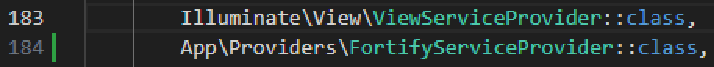
\includegraphics[width=0.5\textwidth]{figures-C1/config_app.pdf}
\end{wrapfigure}
Premièrement, ajoutez cette ligne dans \linebreak \verb|config/app.php|, dans la liste des \verb|providers| utilisés par \laravel{}.

\begin{wrapfigure}[8]{r}{0.5\textwidth}
    \vspace{-0.5cm}
    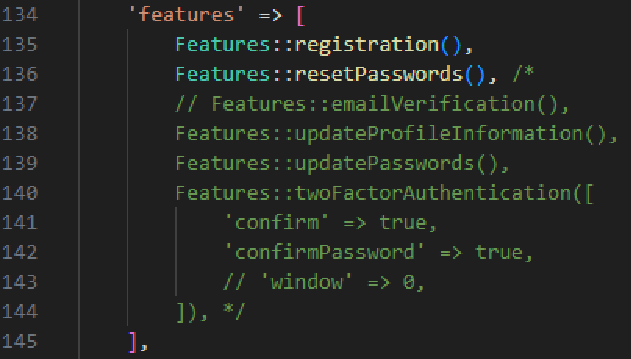
\includegraphics[width=0.5\textwidth]{figures-C1/config_fortify.pdf}
\end{wrapfigure}

Ensuite, dans \verb|config/fortify.php|, ajoutez \verb|/* */| pour commenter les éléments comme ci-contre. L'array \verb|features| permet de dire à \fortify{} quelles fonctionnalités vous souhaitez activer. En l'occurence, nous sommes intéressés par \verb|registration()| et \verb|resetPasswords()|. Voici la liste des fonctionnalités:

\begin{itemize}
    \item \verb|registration()| permet l'authentification de base (register/login).
    \item \verb|resetPasswords()| permet de réinitialiser son mot de passe.
\end{itemize}

\begin{itemize}[resume, before = \vspace*{-0.63cm}]
    \item \verb|emailVerification()| permet de vérifier les adresses emails des utilisateurs.
    \item \verb|updateProfileInformation()| permet de modifier son profil.
    \item \verb|updatePassword()| permet de modifier son mot de passe depuis son profil. 
    \item \verb|twoFactorAuthentification| permet d'activer la double authentification.
\end{itemize}

Ensuite, il faut dire à \fortify{} quelles \views{} correspondent à quelles \routes{}. Pour cela, ajoutez ceci dans \verb|app/Providers/FortifyServiceProvider.php|, plus précisément dans la méthode \verb|boot()|:

\begin{figure}[!h]
    \centering
    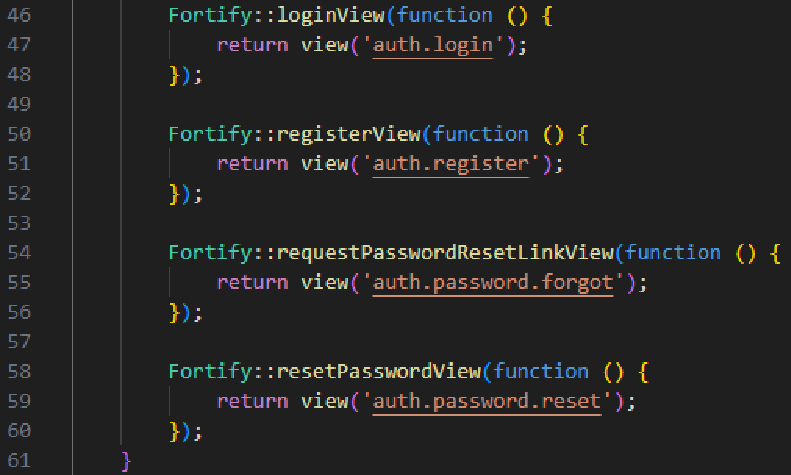
\includegraphics[width=0.75\textwidth]{figures-C1/fortify_provider.pdf}
\end{figure}


\subsubsubsection{Views}
Ensuite, il faut évidement créer les views pour les fonctionnalités que nous gardons. Comme elles sont (très) longues et proviennent d'un package qui n'est plus officiellement supporté (\href{https://github.com/laravel/ui}{Laravel UI}), vous pouvez les trouver ici: \url{https://github.com/nhitec/Laravel-tutorial-auth-blades}. Placez le dossir \verb|auth| dans \verb|resources/views|, et le tour est joué!\footnote{Remarquez que nous n'avons eu besoin ni de \controllers{} ni de \routes{}. C'est parce qu'ils sont déjà créés pour nous. Pour votre curiosité, vous pouvez trouver les \routes{} créées par \fortify{} dans le fichier \verb|vendor/laravel/fortify/routes/routes.php|.}

Afin d'accéder à ces nouvelles pages, il faut que l'on modifie nos boutons dans \verb|index.blade.php|. Nous allons ajouter les \routes{} aux deux bouttons existants, et en rajouter un troisème pour se déconnecter:

\begin{figure}[!h]
    \centering
    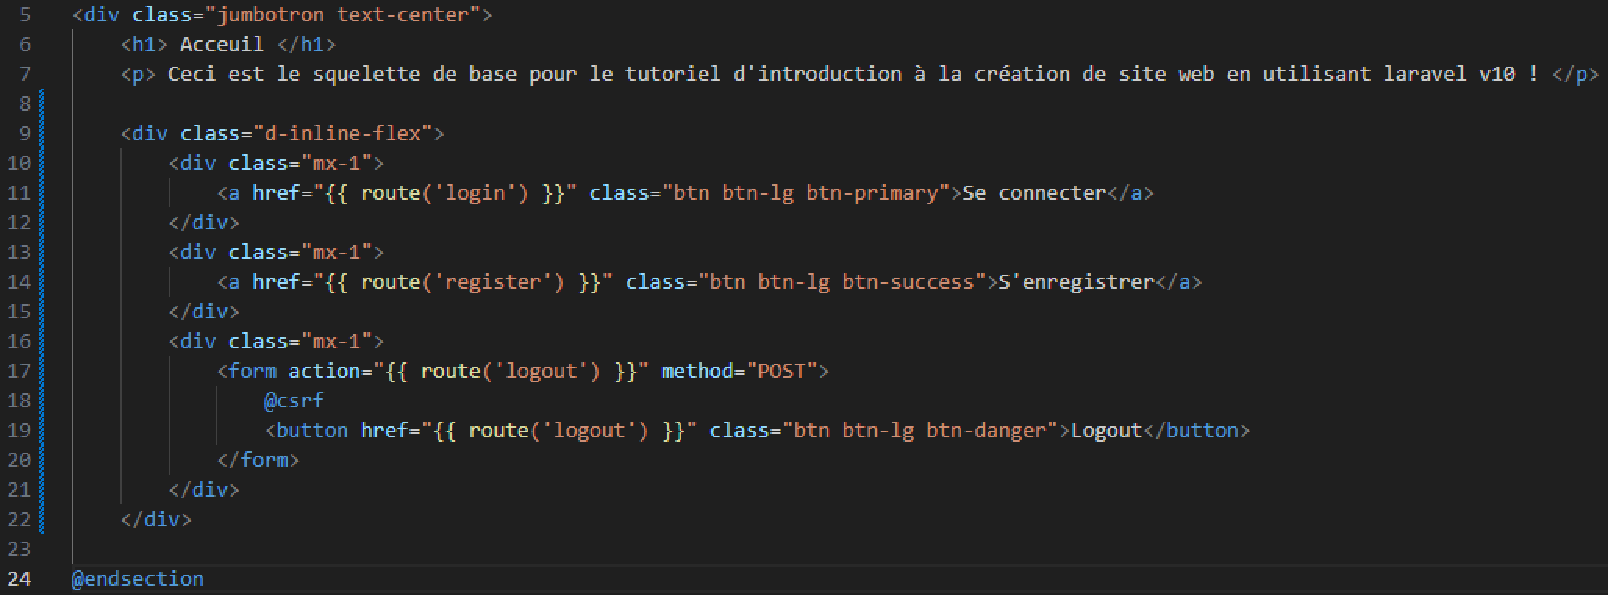
\includegraphics[width=0.75\textwidth]{figures-C1/index_auth.pdf}
\end{figure}

\newpage

Voici les pages que vous devriez obtenir:

\begin{figure}[!h]
    \begin{subfigure}[c]{0.73\textwidth}
        \fbox{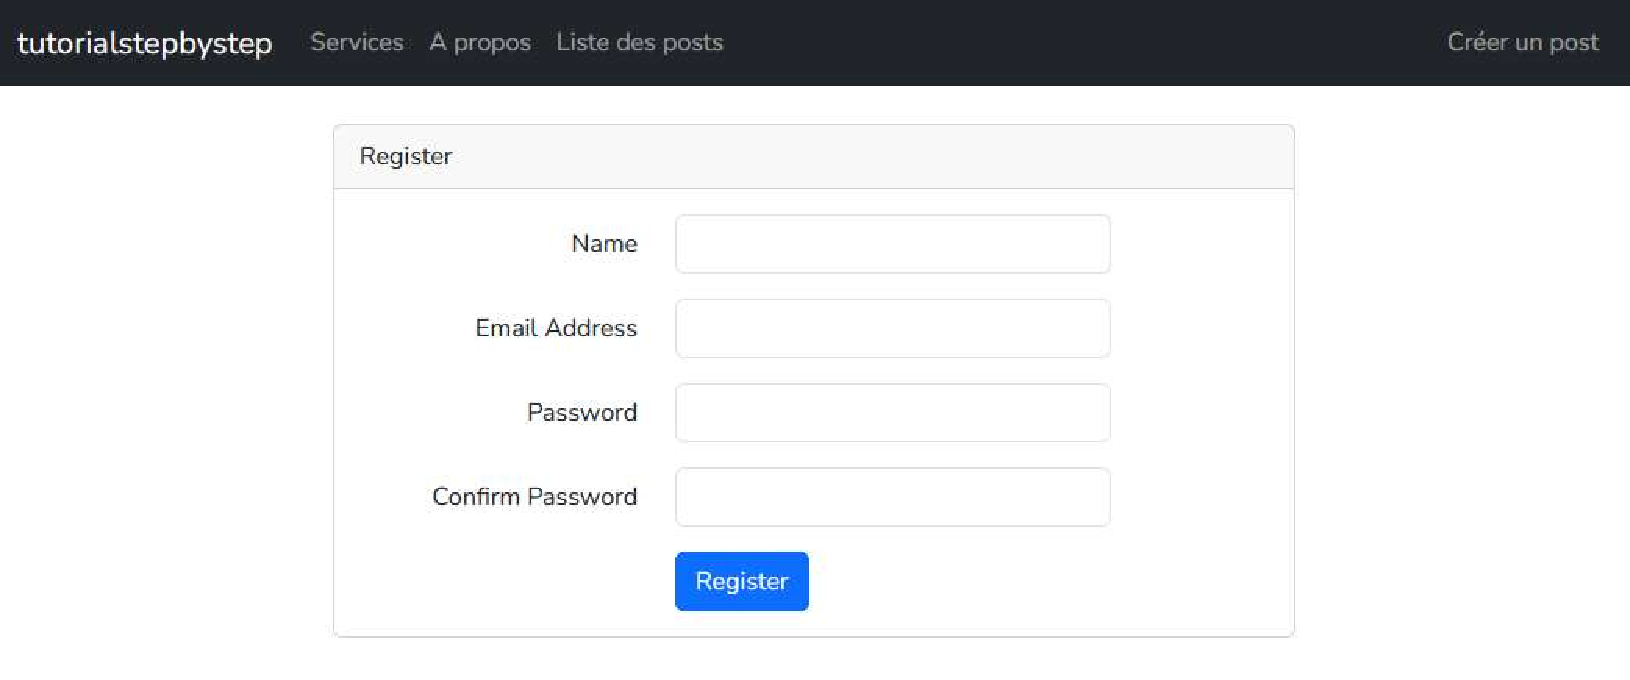
\includegraphics[width=\textwidth]{figures-C1/auth_register.pdf}}
    \end{subfigure}\hfill
    \begin{subfigure}[c]{0.24\textwidth}
        \caption{\url{http://tutorialstepbystep/register}} 
    \end{subfigure}
    \begin{subfigure}[c]{0.73\textwidth}
        \fbox{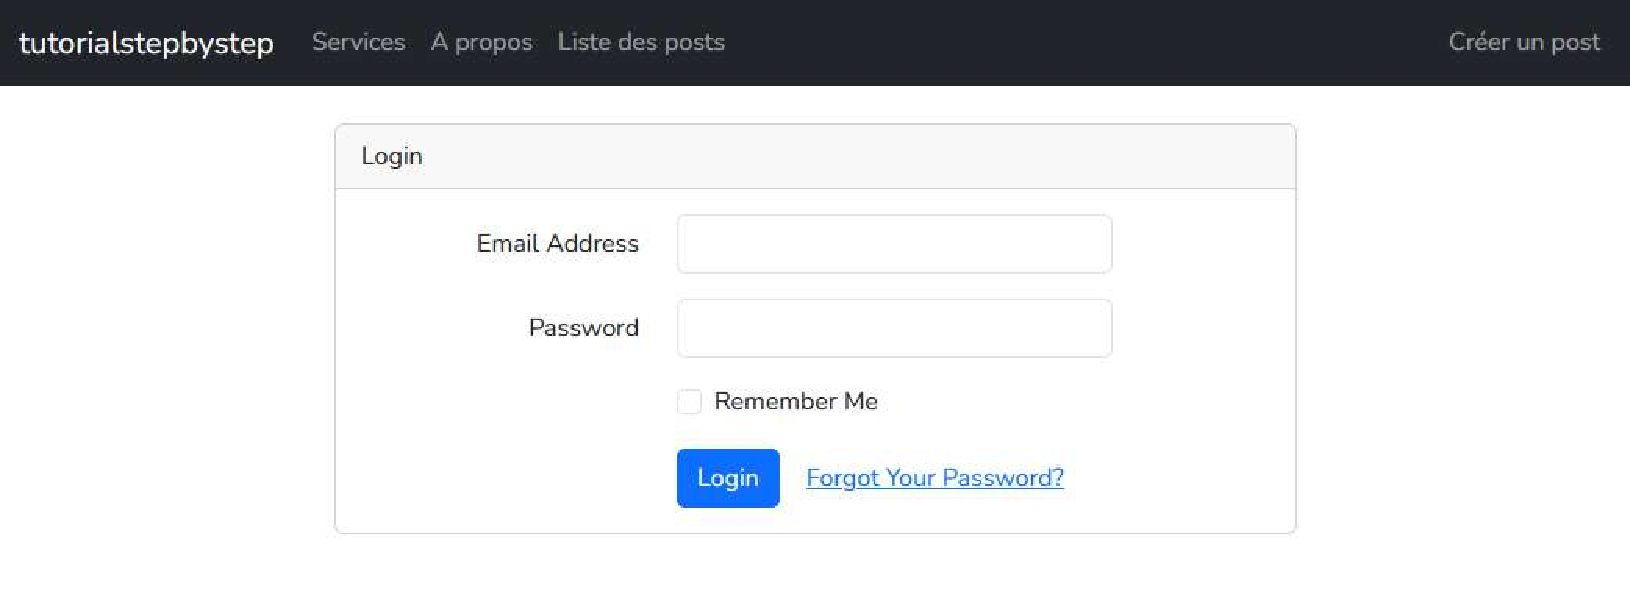
\includegraphics[width=\textwidth]{figures-C1/auth_login.pdf}}
    \end{subfigure}\hfill
    \begin{subfigure}[c]{0.24\textwidth}
        \caption{\url{http://tutorialstepbystep/login}} 
    \end{subfigure}
    \begin{subfigure}[c]{0.73\textwidth}
        \fbox{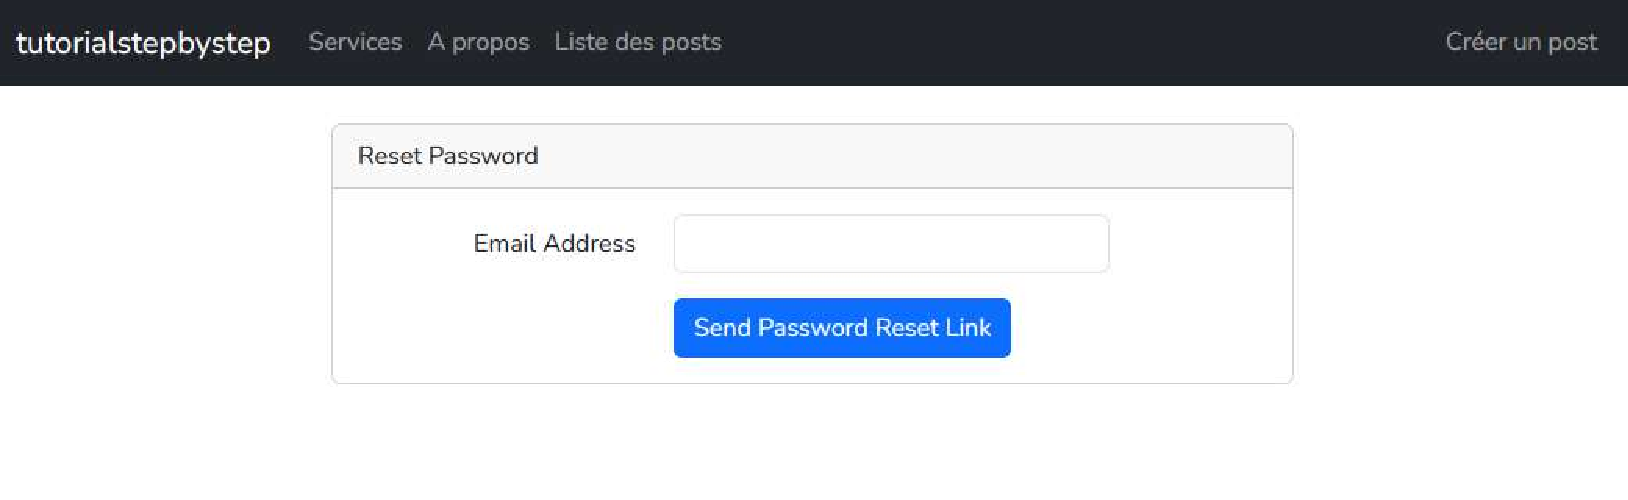
\includegraphics[width=\textwidth]{figures-C1/auth_reset.pdf}}
    \end{subfigure}\hfill
    \begin{subfigure}[c]{0.24\textwidth}
        \caption{\url{http://tutorialstepbystep/forgot-password}\label{fig:auth_forgot}} 
    \end{subfigure}
    \caption{Les quatres pages de gestions des posts.}
\end{figure}

\newpage

Remarquez que le bouton de la \texttt{Figure~\ref{fig:auth_forgot}} ne fonctionne pas, nous règlerons ce problème dans une future \texttt{Section~(WIP)}.

\subsubsection[Middlewares][laravel.com/docs/10.x/middleware]{Middlewares}

Nous arrivons à la fin! La dernière chose à faire, c'est protéger quelques \routes. En effet, il est préférable que n'importe qui ne puisse pas accéder aux posts sans s'être préalablement authentifié. Il faut donc trouver un moyen de vérifier si un utilisateur est connecté avant de lui donner accès à la gestion/création de posts. C'est exactement à cela que servent les \middlewares{}.

De manière générale, les \middlewares{} sont des fonctions qui seront exécutées ``entre deux requêtes'', pour par exemple interdire d'accès une certaine \route{} et rediriger l'utilisateur selon certaines conditions.

Les \middlewares{} se trouvent dans le dossier \verb|app/Http/Middleware| et sont configurés par le fichier \verb|app/Http/Kernel.php|. Les \middlewares{} que nous pouvons assigner manuellement aux \routes{}/\controllers{} sont ceux listés dans \verb|$middlewareAliases|.

En ce qui nous concerne, le \middleware{} \verb|'auth'| est celui qu'il nous faut. Nous allons donc l'ajouter à aux \routes{} responsables des posts dans \verb|routes/web.php| comme cela:

\begin{figure}[!h]
    \centering
    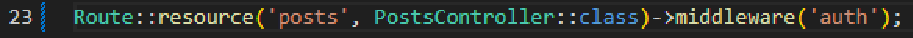
\includegraphics[width=0.75\textwidth]{figures-C1/middleware_auth.pdf}
\end{figure}

Et voilà! Désormais, lorsque vous essayez de voir ou de créer un post sans être connecté, vous devriez vous faire rediriger vers la page de connection.

\newpage